% LaTeX file for resume 
% This file uses the resume document class (res.cls)

\documentclass{res} 
\usepackage{CJK}
\usepackage{enumerate}
\usepackage{url}
\usepackage{graphicx}
\usepackage{wrapfig}
%\usepackage{helvetica} % uses helvetica postscript font (download helvetica.sty)
%\usepackage{newcent}   % uses new century schoolbook postscript font 
\setlength{\textheight}{9.5in} % increase text height to fit on 1-page 

\begin{document} 
\begin{CJK}{UTF8}{bsmi}
\name{Yu-Ching Lin\\[12pt]}     % the \\[12pt] adds a blank
				        % line after name      

\begin{resume}

\begin{wrapfigure}{hr}{30mm}
	\vspace{-1in}
		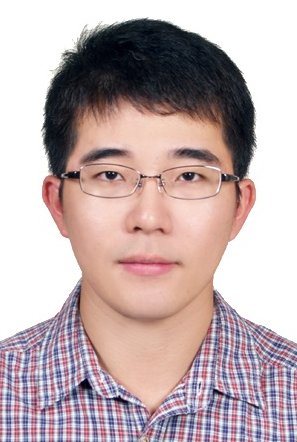
\includegraphics[width=25mm]{head.jpg}
\end{wrapfigure}

\section{Basic Information}
	Birthday: 1984 / 9 / 8  \\
	cell: 0921895172 \\
	E-mail: vagante@gmail.com \\
	personal website: \url{http://mpac.ee.ntu.edu.tw/~vagante}\\

\section{Education}
	\vspace{-0.1in}
	\begin{tabbing}
	\hspace{0.3in}\= \hspace{4.6in}\= \kill
	\textbf{Master}, Communication Engineering, National Taiwan University \>\>2007.09 - 2009.06 \\
		\>Overall grade average: 90.86 (the score of master thesis: 91.80)\\	
	\textbf{Bachelor of Science}, Electrical Engineering, National Taiwan University  \>\>2003.09 - 2007.06 \\
		\>Overall grade average: 83.27, overall GPA: 3.62 / 4.00. \\
    Taipei Nunicipal Jianguo High School                     \>\>2000.09 - 2003.06 \\
	\end{tabbing}\vspace{-20pt}

 
\section{Work Experiences}
   \vspace{-0.1in}	
   \begin{tabbing}
   \hspace{0.3in}\= \hspace{4.6in}\= \kill % set up two tab positions
	\underline{\textbf{Military Service}} in National Army of Taiwan, R. O. C.             \>\>2009.10 - 2010.9 \\
	\underline{\textbf{Research Assistent}} of Pro. Homer H. Chen                          \>\>2007 - 2009 \\
	\underline{\textbf{Reviewer}} of ACMMM '09 and ICIP '08              \>\>2008, 2009 \\
	\underline{\textbf{Research Assistent}} of Spoken Language Group in Academic Sinica     \>\>2007.07 - 2007.09 \\
	\underline{\textbf{Administrative Assisitent}} of Little Giant Chinese Chamber Orchestra    \>\>2005 - 2007 \\
	\underline{\textbf{Leader}} of National Taiwan University Chinese Orchestra              \>\>2005 - 2006 \\
   \end{tabbing}\vspace{-20pt}      % suppress blank line after tabbing

\section{Research Field}
	Audio and video signal processing, Multimedia analysis and indexing, \\Data mining, Machine learning \\

\section{Skills}          
	Programming: C, C++, JAVA, Python, Matlab, Objective C \\
	IDE: Visual Studio, Xcode, Eclipse, Vim \\
	OS: Windows, Linux, MAC \\

\section{Honor}         
	\vspace{-0.1in}
	\begin{tabbing}
	\hspace{0.3in}\= \hspace{4.6in}\= \kill
	Third place in the NISSAN Design Award held by Nissan Taiwan \>\>2007 \\
	\> An annual contest for novel electrical equipment or technology on vehicle \\
	\end{tabbing}\vspace{-20pt}

\section{Publication}
	\vspace{-0.1in}
	\subsection{Journal}
		\begin{enumerate}[1.~]
			\item \textbf{Y.-C. Lin}, Y.-H. Yang, and H.-H. Chen, 
				``Exploiting online music tags for emotion classification,''
				submitted to ACM Transactions on Multimedia Computing, Communications and Applications (ACM TOMCCAP).
			\item Y.-H. Yang, \textbf{Y.-C. Lin}, Y.-F. Su, and H.-H. Chen, 
				``A regression approach to music emotion recognition,'' 
				IEEE Trans. Audio, Speech and Language Processing (TASLP), 
				vol. 16, no. 2, pp. 448-457, Feb. 2008.
		\end{enumerate}	
	\subsection{Conference}
		\begin{enumerate}[1.~]
			\item Y.-H. Yang, \textbf{Y.-C. Lin}, and H.-H. Chen, 
				``Personalized music emotion retrieval,'' 
				Proc. ACM Int. Conf. Information Retrieval (SIGIR), 
				pp. 748–749, 2009.
			\item Y.-H. Yang, \textbf{Y.-C. Lin}, A. Lee, and H.-H. Chen, 
				``Improving musical concept detection by ordinal regression and context fusion,'' 
				Proc. Int. Conf. Music Information Retrieval (ISMIR), 
				pp. 147–152, 2009.
			\item M.-Y. Su, Y.-H. Yang, \textbf{Y.-C. Lin}, and H.-H. Chen, 
				``An integrated approach to music boundary detection,'' 
				Proc. Int. Conf. Music Information Retrieval (ISMIR), 
				pp. 705–710, 2009.
			\item Y.-H. Yang, \textbf{Y.-C. Lin}, and H.-H. Chen, 
				``Clustering for music search results,''
				Proc. IEEE Int. Conf. Multimedia and Expo (ICME), 
				pp. 874–877, 2009.
			\item \textbf{Y.-C. Lin}, Y.-H. Yang, and H.-H. Chen, 
				``Exploiting genre for music emotion classification,''
				Proc. IEEE Int. Conf. Multimedia and Expo (ICME), 
				pp. 618–621, 2009.
			\item H.-T. Cheng, Y.-H. Yang, \textbf{Y.-C. Lin}, and H.-H. Chen, 
				``Multimodal structure segmentation and analysis of music using audio and textual information,'' 
				Proc. IEEE Int. Symp. Circuits and Systems (ISCAS), 
				pp. 1677–1680, 2009.
			\item Y.-H. Yang, \textbf{Y.-C. Lin}, H.-T. Cheng, and H.-H. Chen, 
				``Mr.Emo: Music retrieval in the emotion plane,'' 
				Proc. ACM Int. Conf. Multimedia (SIGMM), technical demonstration, 
				pp. 1003–1004, 2008.
			\item Y.-H. Yang, \textbf{Y.-C. Lin}, H.-T. Cheng, I.-B. Liao, Yeh-Chin Ho, and H.-H. Chen, 
				``Toward multi-modal music emotion classification,''
				Proc. Pacific-Rim Conf. Multimedia (PCM), 
				pp. 70–79, 2008.
			\item H.-T. Cheng, Y.-H. Yang, \textbf{Y.-C. Lin}, I.-B. Liao, and H.-H. Chen, 
				``Automatic chord recognition for music classification and retrieval,'' 
				Proc. IEEE Int. Conf. Multimedia and Expo (ICME), 
				pp. 1505–1508, 2008.
			\item Y.-H. Yang, Y.-F. Su, \textbf{Y.-C. Lin}, and H.-H. Chen, 
				``Music emotion recognition: The role of individuality,''
				Proc. ACM Int. Workshop on Human-centered Multimedia (ACM HCM), 
				pp. 13–21, 2007.
			\item Y.-H. Yang, \textbf{Y.-C. Lin}, Y.-F Su, and H.-H. Chen, 
				``Music emotion classification: A regression approach,''
				Proc. IEEE Int. Conf. Multimedia and Expo (ICME), 
				pp. 208–211, 2007.
		\end{enumerate}
	\subsection{Patent}
		\begin{enumerate}[1.~]
			\item Y.-C. Lin et al, “A genre-based two-layer structure for music emotion classification,” Taiwan pending.
		\end{enumerate}

\section{Courses}
	\vspace{-0.1in}
	\subsection{Master}
		\begin{itemize}
			\item Video processing: Digital Visual Effects
			\item Multimedia indexing: Data mining, Advanced multimedia analysis and indexing, Web mining
			\item Algorithm: Genetic Algorithm, Machine learning, Multivariate analysis
		\end{itemize}

	\subsection{Bachelor}
		\begin{itemize}
			\item Basic: Electronics, Electromagnetism, Circuits, Engineering Mathematics, Computer programing, Computer science, Switching Circuit and Logic Design
			\item Communication: Signal processing, Communication theory, Networking
			\item Computer: Data structure, Object oriented programming, Algorithm
			\item Video processing: Computer vision
			\item Signal processing: Digital signal processing, Digital speech processing
			\item Multimedia indexing: Pattern recognition, Multimedia analysis and indexing
			\item Experiment: Network and multimedia experiment
			\item Others: Linear system, Control system, Microwave system
		\end{itemize}

\section{Master thesis}
	Advisor: Prof. Homer H. Chen \\
	Title: Exploiting Metadata for Music Emotion Classification \\
	Abstract:\\

Along with the explosive growth of the social tagging systems and musical web services,
abundant musical metadata are readily obtainable from the Internet.
Since most metadata are related to the human perception of music, 
they can be utilized to bridge the so-called semantic gap 
between audio signals and high-level semantics for content-based music classification. 
In this thesis, we first examine the correlation between 
emotion and the musical metadta by a statistical association test,
and then exploit such correlation for emotion classification.
We propose to divide songs according to the metadata and 
build a metadata-specific model to concentrate on the classification in each group.
Since a song can be associated with differen types of metadata, such as genre and style,
we further propose a novel adaptive fusion scheme to utilize all types of metadata. 
While the existing methods of exploiting metadata are hampered 
by the noise and sparseness inherent to metadata, 
the proposed scheme overcomes these difficulties and 
significantly improves the accuracy of emotion classification.

\newpage
	\section{Academic report of bachelor degree}
	\vspace{0.3in}
	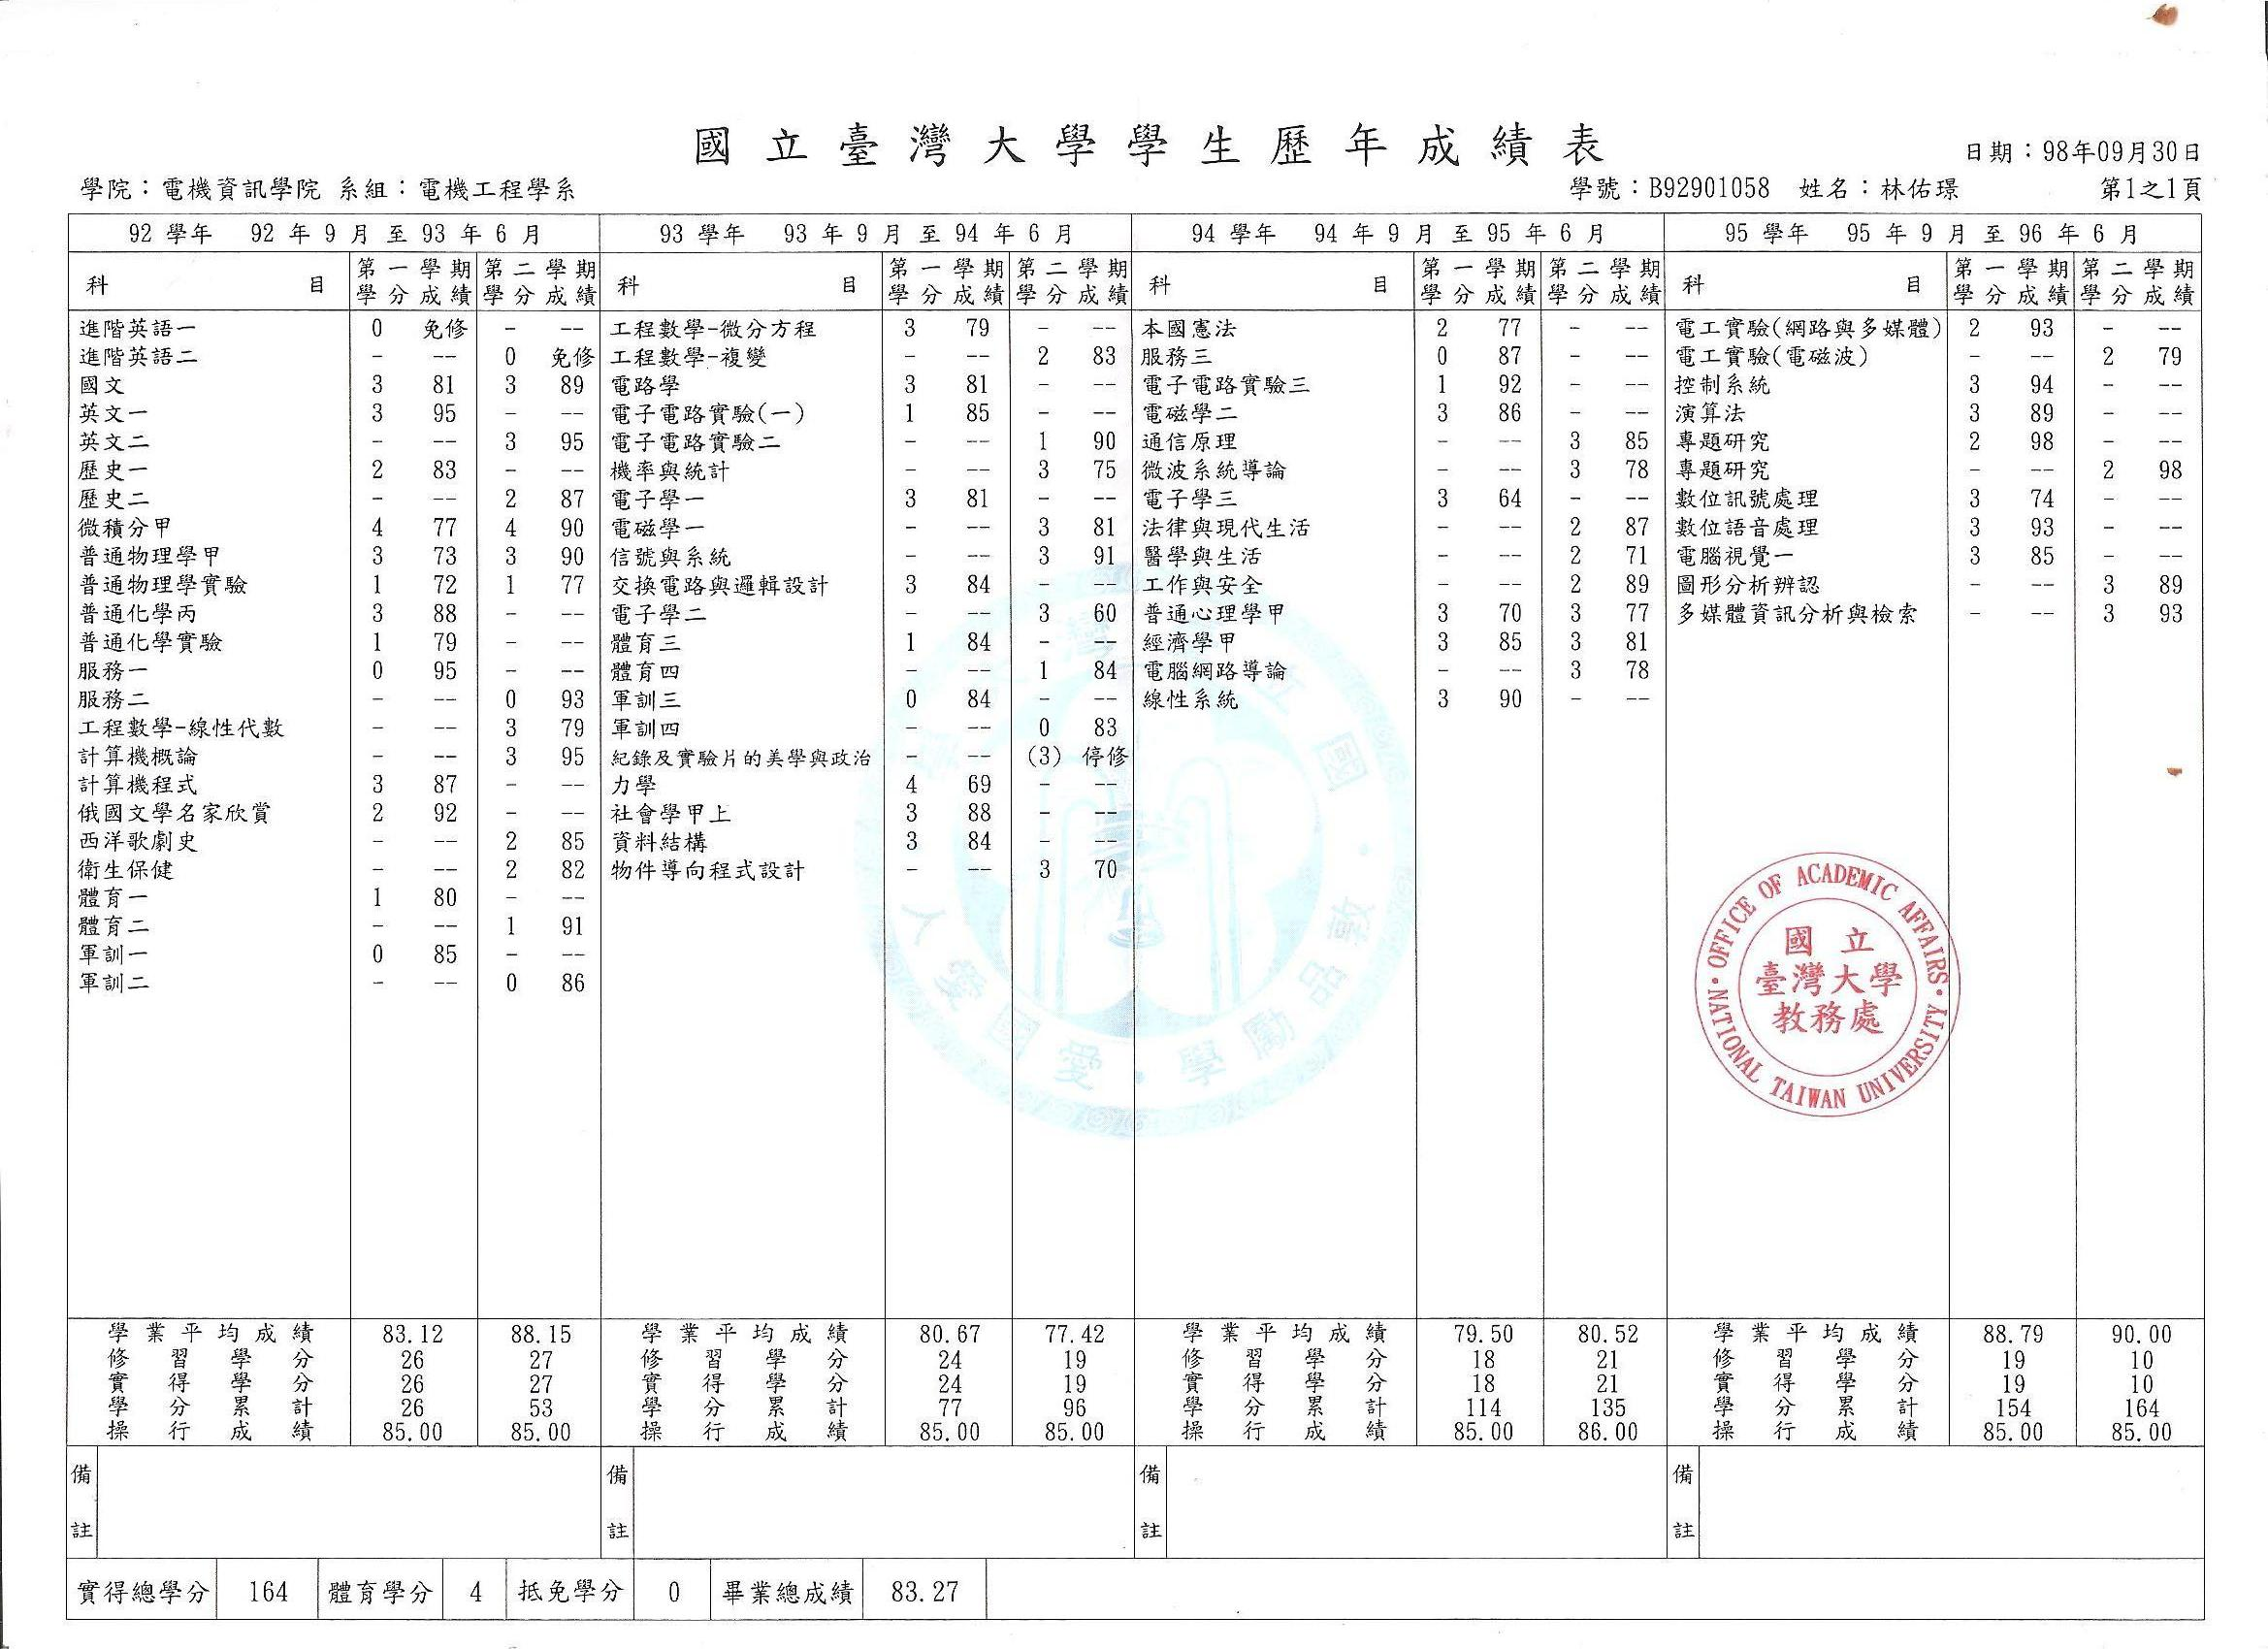
\includegraphics[angle=90,width=\textwidth]{copy1077.jpg}

\newpage
	\section{Academic report of master degree}
	\vspace{0.3in}
	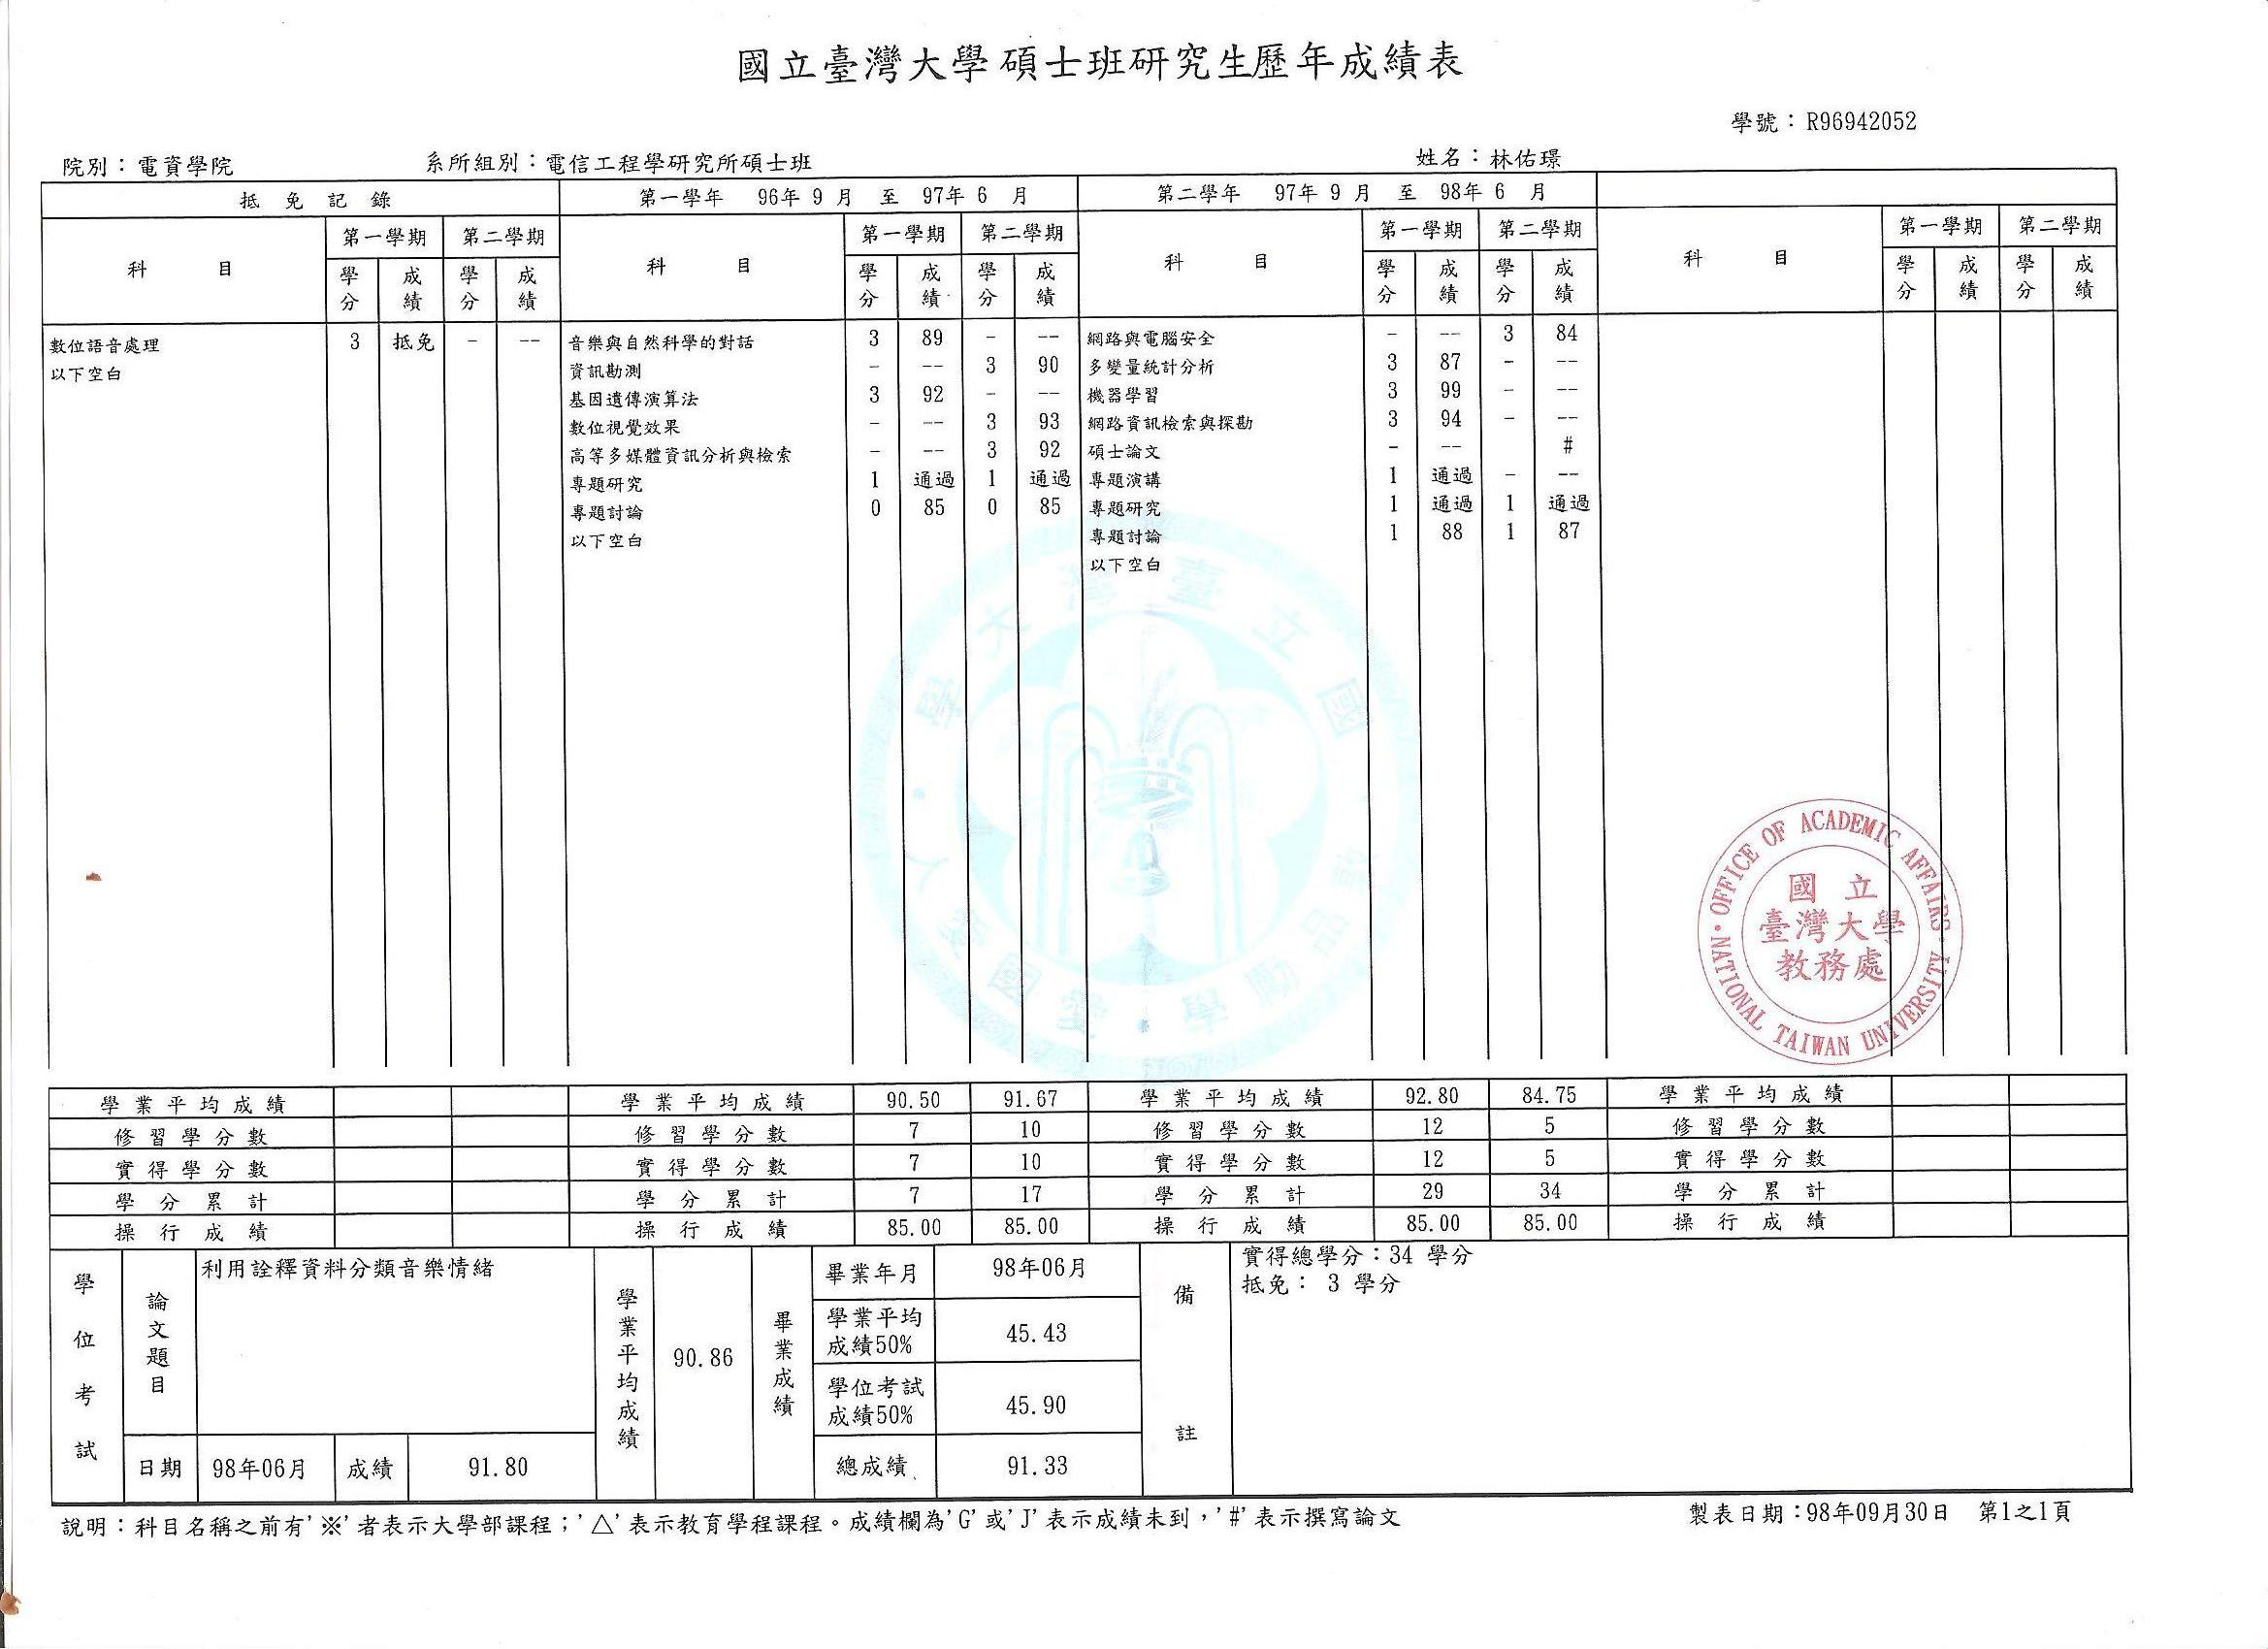
\includegraphics[angle=90,width=\textwidth]{copy1078.jpg}

\end{resume}
\end{CJK}
\end{document}
